%!TEX root = ../main.tex

\chapter{Evaluation}\label{sec:eval}

The difficulty in describing this project's merit stems from its novelty,
being the crescendo of many years of work to make automatic program verification
accessible to any who understand separation logic, not just the authors of
Gillian. The technical hurdles faced during actual implementation are not
especially profound, as the main challenge of this project lied in the
broad and deep prerequisite understanding needed to bring the intricacies of
Gillian together with the more concrete aspects of the DAP, VSCode's extension
API, and modern web development --- all within the limited time span of a MEng
final project. There are very few competing projects in this space; those that
do exist either have significantly different goals (Infer), or exist in a
prototype stage (VeriFast).
\todo{Should this be here or in the conclusion?}

\section{Vs. Previous Gillian Debugging Methods}

Compared to the original debugging method --- manually reading the log file
resulting from verification --- the advantages of the visual debugger are
obvious. Not only does the file log require a deep understanding of Gillian's
internals, but it contains a vast amount of detail, often obfuscating the
information relevant to the encountered error.
Even in the simple case of the recursive list length function, which was used as
a baseline throughout the project, a total of 9328 lines of logging output is
generated during verification. As a more precise comparison, about 1500 of those
lines concern unification of the postconditions, with a high degree of
redundancy and verbosity. This contrasts with what is essentially a few lines of
text in the debugger interface, with more detail available as and when the user
requires. Compared to the clear, clean, and concise interface of the new
solution, a far more ideal debugging process has been presented --- even those
with a deep understanding of Gillian, who are well acclimated to debugging via
the file log, intend to use this as their primary method of debugging moving
forwards.

The new debugger is also leaps and bounds ahead of the previous iteration;
aside from not having any unification information whatsoever, its use requires
a user to understand some of the quirks of the solution, such as branches
being executed one after the other with no means of discerning between then.
The first debugger was very much a case of attempting to move Gillian a step
closer to debugging in whatever manner was available, rather than setting out a
clear vision of what prospective users would desire from a program verification
debugger, and working to meet that goal.


\section{Vs. VeriFast}

VeriFast has a fundamentally different approach to the debugging process;
instead of reporting the results of symbolic execution step by step, the whole
verification is performed all at once, only showing details in the event of an
error (or a breakpoint being reached). There is no concept of exploring the
different execution paths of the program, severely limiting its ability to be
used as a tool for deepening one's understanding of separation logic. Multiple
branches of execution are not presented to the user, only showing the single
path taken to reach the error or breakpoint. Compare this rigid textual format
to the Gillian debugger's explorable execution map in
\autoref{fig:verifast-path-compare}; not only is the latter more feature rich,
it gives a full view of the program execution.

\begin{figure}
  \centering
  \begin{subfigure}[b]{0.4\textwidth}
    \center{}
    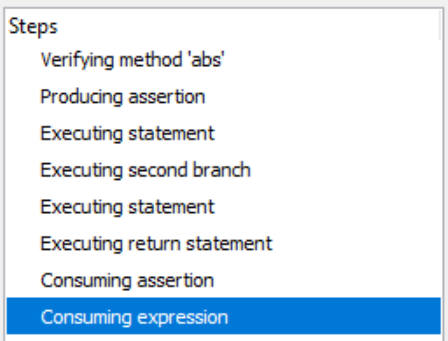
\includegraphics[width=0.75\textwidth]{img/verifast-path.png}
    \caption{The execution path information given by VeriFast}%
    \label{fig:verifast-path}
  \end{subfigure}
  \qquad
  \begin{subfigure}[b]{0.4\textwidth}
    \centering
    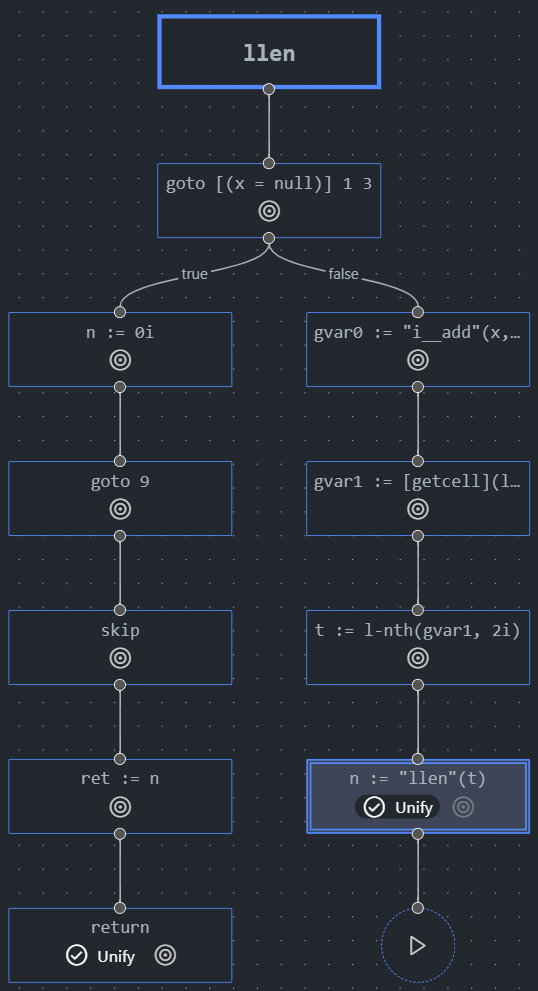
\includegraphics[width=0.9\textwidth]{img/execmap-final.png}
    \caption{The Gillian debugger's execution map}%
    \label{fig:execmap-final}
  \end{subfigure}
  \caption{Comparison of branch information given by VeriFast and the Gillian
  debugger respecitvely}%
  \label{fig:verifast-path-compare}
\end{figure}

VeriFast also gives no insight into the unification process; the only
information provided is an error message should unification fail. The Gillian
debugger gives more information to this end by showing all assertions from
a unification, up to and including the failing one.

\begin{figure}
  \centering
  \begin{subfigure}[b]{0.4\textwidth}
    \center{}
    
\includegraphics[width=0.9\textwidth]{img/verifast-error.png}
    \caption{A unification error given by VeriFast}%
    \label{fig:verifast-error}
  \end{subfigure}
  \qquad
  \begin{subfigure}[b]{0.4\textwidth}
    \centering
    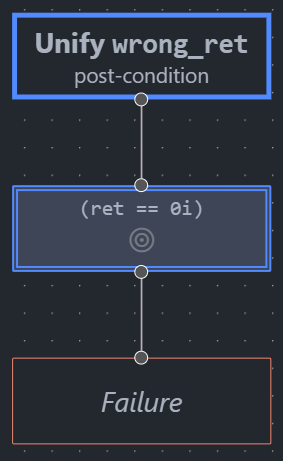
\includegraphics[width=0.3\textwidth]{img/unifymap-failure.png}
    \caption{A failing unification map given by the Gillian debugger}%
    \label{fig:unifymap-failure}
  \end{subfigure}
  \caption{Comparison of information for a failing unification, given by
  VeriFast and the Gillian debugger respectively}%
  \label{fig:verifast-unifyfail-compare}
\end{figure}

Another point of comparison is the accessibility of the different solutions.
VeriFast is a completely isolated tool, its graphical interface needing to be
run separately from any other software used for development. Now, armed with the
new debugging functionality, developers have a real possibility of using Gillian
as part of their development pipeline; the ability to debug Gillian verification
directly inside what is, by far, the most popular editor in the world is a
previously unmatched level of accessibility for a tool of this purpose.


\section{Limitations}%
\label{sec:eval:limitations}

There are some features that are desired of a Gillian debugger that are not yet
present, including:
\begin{itemize}
  \item Full support for target language lifting
  \item Decorating the source code during debugging
  \item Highlighting the relevant blocks of memory for the selected assertion
        when inspecting unification
  \item More efficient database logging
  \item A query language for the execution and unification trees
\end{itemize}

However, all of these features are either relatively trivial to implement and
only missing due to time constraints, or more experimental features that require
substantial planning and are far outside the scope of this project.

Of course, none of that detracts from the fact that this project has elevated
Gillian from a prototype research tool to one that that proves useful in
pursuing new research in separation logic, and even more impressively, a tool
that can be used for educational purposes --- to help those having their first
experience of separation logic form a deeper understanding by automatically
applying its principles to real programs.
